\section{Architecture}
Maestro is organized as a pipeline that processes the program and its input from a file, or from a REPL, and interprets the code. Figure \ref{fig:archi} gives a high level overview of Maestro's architecture.
In the next sections, we present the interfaces between different parts of our interpreter, and then describe each module.

\begin{figure}[h!]
  \centering
  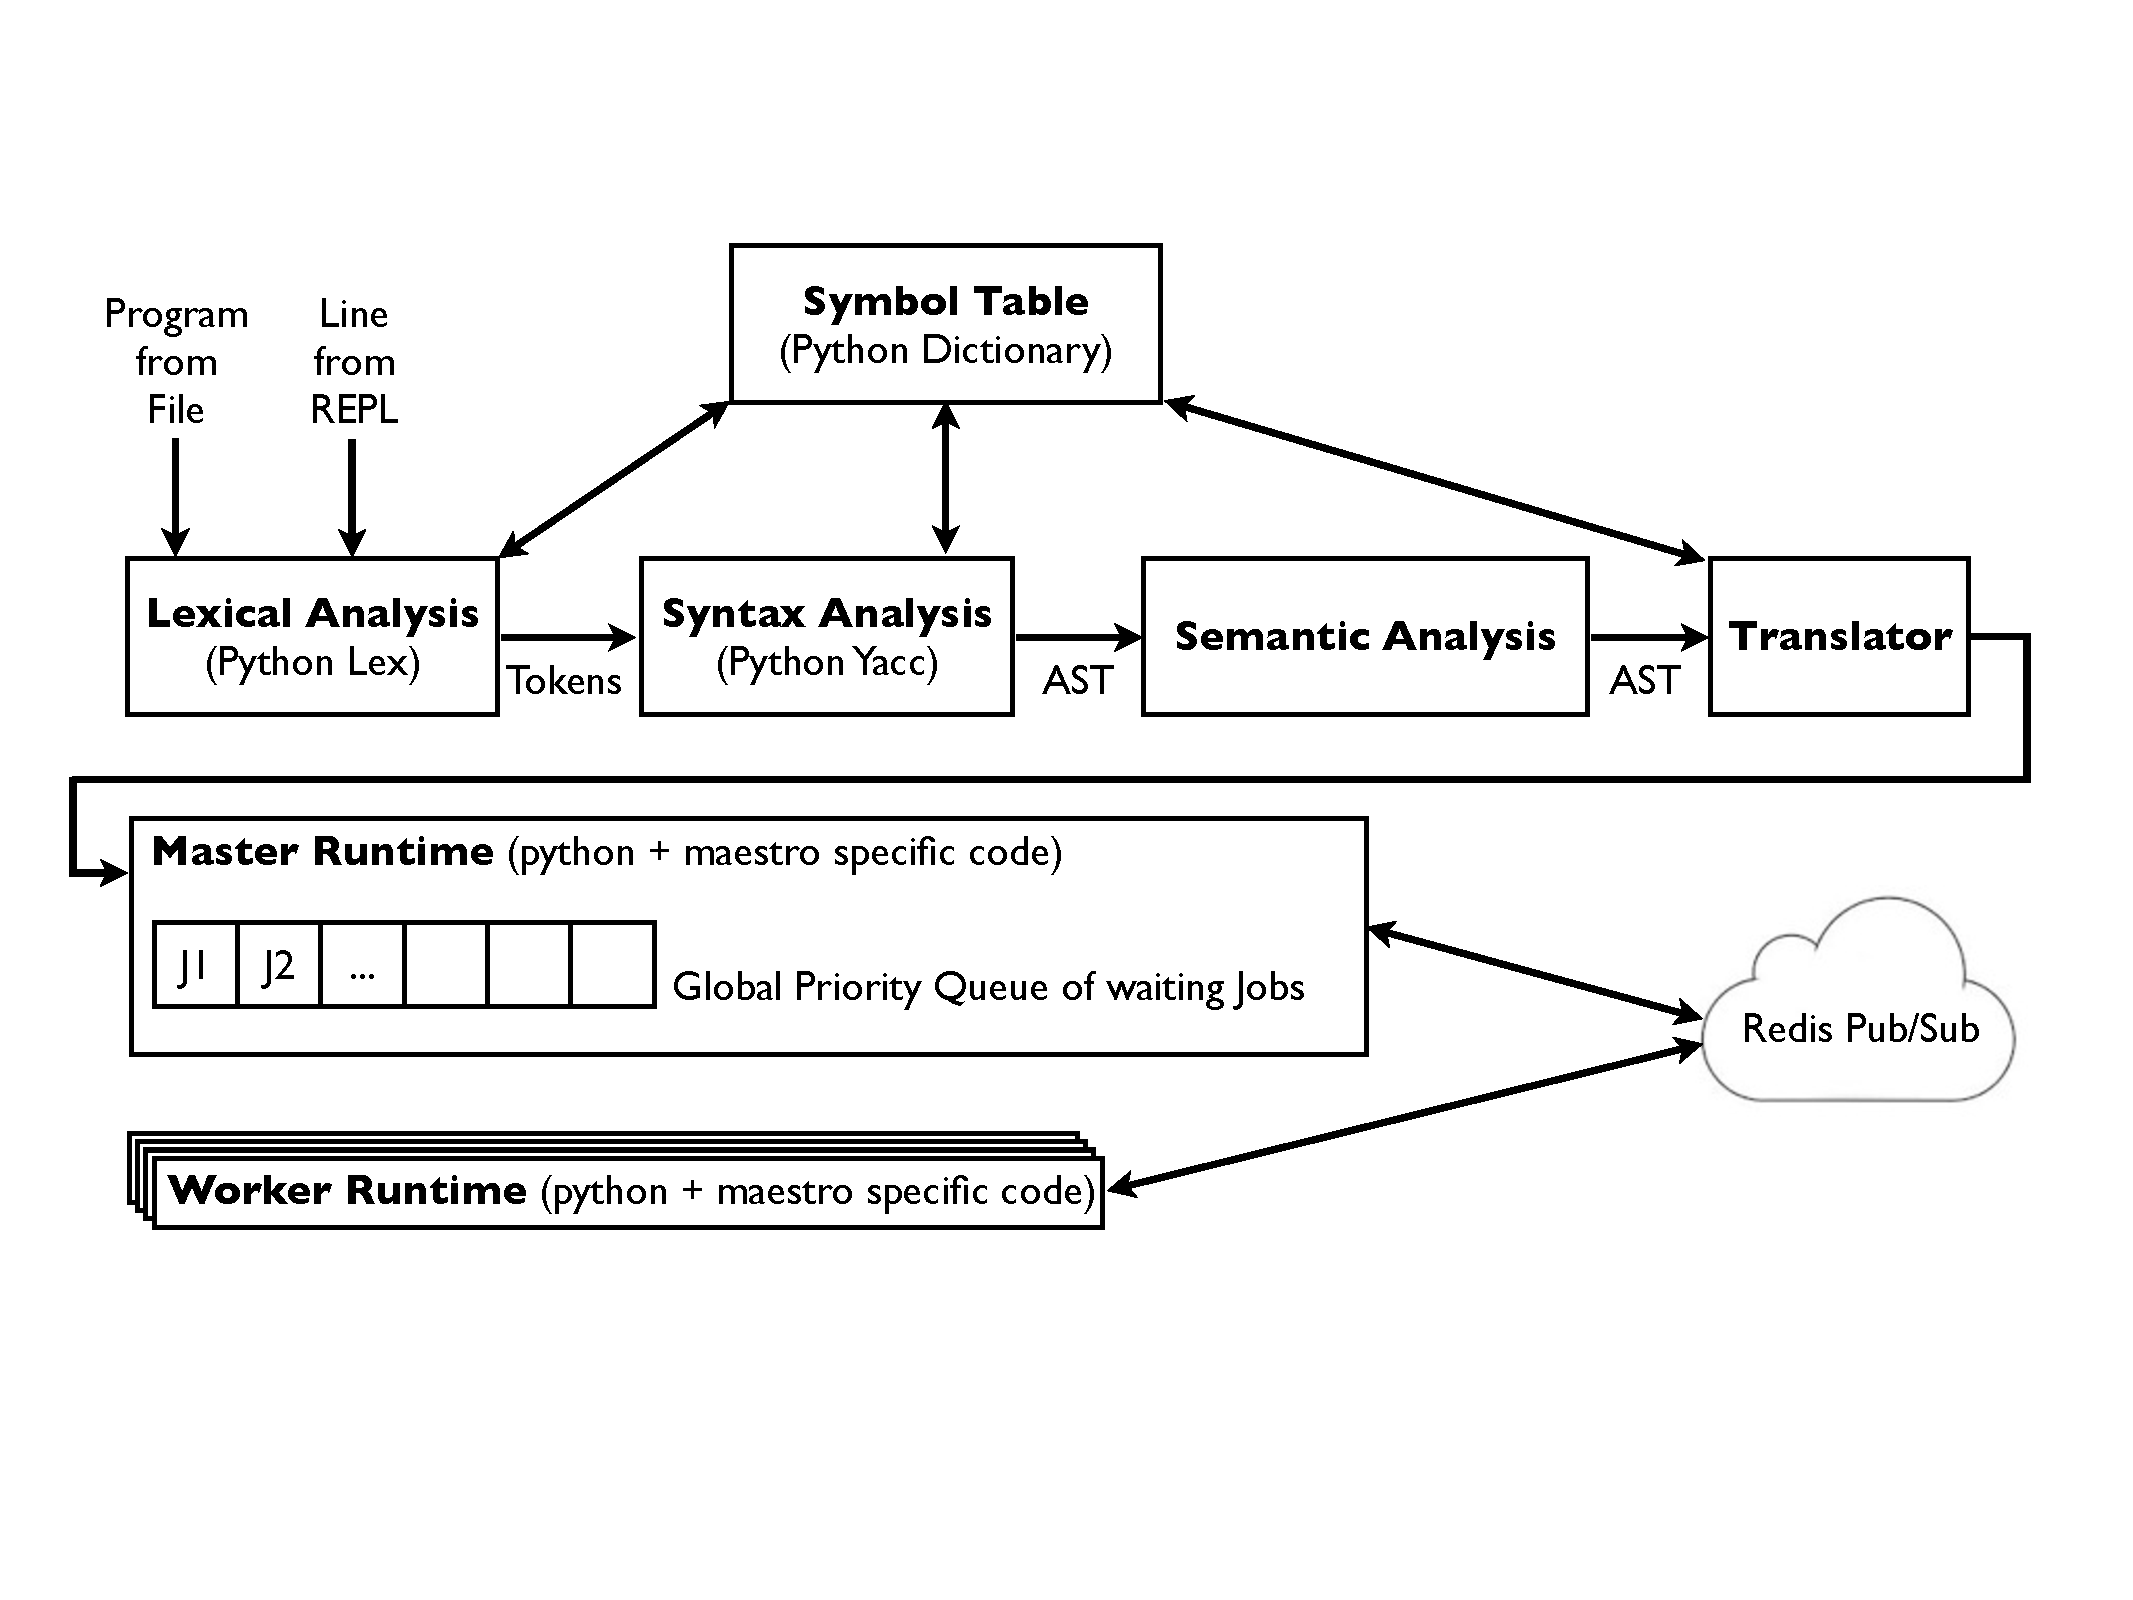
\includegraphics[width=15cm]{figures/archi.pdf}
  \caption{Maestro Architecture}
\label{fig:archi}
\end{figure}

\section{Interfaces}
The two main interfaces are the AST and the API. We will describe them in turn.

\paragraph{AST}

The AST is produced by the syntax analyser.
It is a tree with each node having children, or a value if it is itself a leaf.
The node also comprises the type of the expression it represents.
It is used by the syntax analyser and the translator.

\paragraph{API}

The API is exposed by the backend, and gives Maestro-specific features to the translator.
In particular, it exposes a Job object, central to our language, and functions to set dependencies and add Jobs
to the run queue.

\section{Modules}

\paragraph{Lexer}

The lexer takes the program or the REPL lines, and produces tokens for the syntax analyser.
Comments are discarded by the lexer directly.

The Lexer was written by Mathias with PLY.

\paragraph{Syntax Analyser}

The Syntax Analyser contains the grammar for Maestro, and uses the lexer's output to produce the AST using bottom-up parsing and an S-attribute SDD.

The Syntax Analyser was written with PLY. Mathias wrote the grammar and SDD and Georgios handled error recovery.

\paragraph{Semantic Analyzer}

The Semantic Analyser walks the AST to verify type compatibility and that variables were declared before being accessed.

The Semantic Analyser was written by Georgios.

\paragraph{Translator}

The translator translates the AST into Python and executes it.
It is coded as a recursive function that keeps track of computed values and types.
It makes extensive use of the backend API for Job creation and management, and leverages python expressiveness to implement complex features like map/reduce and dynamic code dependencies.

The translator was written by Mathias.

\paragraph{Backend}

The Backend exposes Maestro specific abstraction and handles the Job scheduling and distribution.
Because it's fairly complex and interesting,  but doesn't have its own section, we descibe it in more length here.
To support \lang{}'s job scheduling and dispatching for remote execution, we
built a distributed communication protocol whose main components are: (i)
a local job queue, (ii) a Redis
publish/subscribe communication channel, and (iii) a pool of workers dedicated
to job execution. The local job queue is used to keep track of active jobs
and their dependencies and is bound to a runtime environment. A custom Daemon
spins periodically on the job queue and dispatches for execution jobs with
resolved dependencies. Since job execution is either local or remote, job
dispatching is optional. On local execution, the job dispatcher requests a
shell on the local machine for job execution. On remote execution, the job
dispatcher sends requests to check which are the active workers on the Redis
channel, and afterwards dispatches (publishes) a job to the channel. One of the
subscribed active workers executes the job and sends back the output, on a job
specific redis channel. When the runtime Daemon receives the output of the
dispatched job via the job-specific channel, it prints its stdout and also
saves it in a log file under the current working directory.

Most of the Backend code was written by Vaggelis. Georgios and Mathias added some glue and small features.

\paragraph{Testing}:
Testing is a key part of any complex software system.
This is why it was assigned two persons.
Our testing framework will be described in details in a later chapter.

The testing frameworks and most of the tests were written by Arun and Yiren, and integrated from informal tests used by developers of new features.


\section{Organization}
The hard thing with a multi-person project with many parts depending on each other is figuring out a way to all work in parallel.
Even if we didn't always succeed, we took several steps to maximize parallelism.
First, we had an early "hello world" program working by implementing a basic lexer and semantic analyser and a basic backend.
We did not produced an AST and called backend functions directly, but having an end to end program helped a great deal in thinking about more advanced features we wanted.

We then added the production of an AST from the lexical analyser, while still computing values on the fly to keep being able to run programs.
This allowed us to add semantic analysis, and work on the translator that traverses the AST.
When we finally switched to working on a translator, adding features from the backend like remote Jobs was much easier.
